\documentclass{article}


\usepackage{latexsym}
\usepackage{graphicx}
\usepackage{amsmath}
\usepackage[fontset=mac]{ctex}
\usepackage{amsthm,amsmath,amssymb}
\usepackage{mathrsfs}

\title{Numerrical Analysis}
\author{欧阳尚可  3190102458}
\date{\today}

\begin{document}
\maketitle

\newpage
\subsection*{Ex 11.9}
\indent 对于$i=0$我们有$\frac{r}{2}g_0(t_n)=\frac{r}{2}U_0^n;\frac{r}{2}g_0(t_{n+1})=\frac{r}{2}U_0^{n+1}$,因此有$U^{n+1}_1-\frac{r}{2}(U_2^{n+1}-2U_{1}^{n+1})=U_1^n+\frac{r}{2}(U_2^n-2U^n_1)+\frac{r}{2}(g_0(t_n)+g_0(t_{n+1}))\Rightarrow -rU^{n+1}_0+2(1+r)U_1^{n+1}-rU^{n+1}_2=rU^n_0+2(1-r)U^n_1+rU^n_2$这符合Grank-Nicolson方法,同理可知$i=m$时也是符合该方法。对于$i\ne0$且$i\ne m$有$U_i^{n+1}-\frac{r}{2}(U_{i+1}^{n+1}-2U_i^{n+1}+U_{i-1}^{n+1})=U^n_i+\frac{r}{2}(U_{i+1}^n-2U_i^n+U_{i-1}^n)\Rightarrow -rU_{i-1}^{n+1}+2(1+r)U_i^{n+1}-rU_{i+1}^{n+1}=rU^n_{i-1}+2(1-r)U^n_i+rU_{i+1}^n$。

\subsection*{Ex 11.24}
\indent 这里为了方便,我们暂时将记号放到下标,考虑$u^{'}=\lambda u$我们有$\frac{U_{n+1}-U_{n}}{k}=\theta U^{'}_n+(1-\theta)U^{'}_{n+1}=\theta\lambda U_n+(1-\theta)\lambda U_{n+1}\Rightarrow U_{n+1}=\frac{1+k\theta\lambda}{1+k(\theta-1)\lambda}U_n$。要使得其绝对收敛,我们有$\vert \frac{1+k\theta\lambda}{1+k(\theta-1)\lambda}\vert\le1$,化简得到$2k\lambda\le(2\theta-1)k^2\lambda^2$。由Lemma 11.19我们知道特征值都是小于0的,由此我们知道$2\theta-1\ge0\Rightarrow \theta\in[\frac{1}{2},1]$时,对于所有的k,不等式都成立。当$\theta\in[0,\frac{1}{2})$时,有$k\le\frac{h^2}{2(1-2\theta)\nu}$。

\subsection*{Ex 11.40}
\indent 由11.20可以得到$[-\theta rg(\xi)e^{-i\xi h}-\theta rg(\xi)e^{i\xi h}+(1+2\theta r)g(\xi)]U_i^n=[(1-\theta)re^{-i\xi h}+(1-\theta)re^{i\xi h}+(1-2(1-\theta)r)]U_i^n$因此有$g(\xi)=\frac{1-4(1-\theta)rsin^2(\frac{\xi h}{2})}{1+4\theta rsin^2(\frac{\xi h}{2})}$,我们有$\vert g(\xi)\vert\le1$,化简得$rsin^2(\frac{\xi h}{2})\ge2(1-2\theta)r^2sin^4(\frac{\xi h}{2})$,引入r的定义以及平方的非负性我们可以进一步得到$1\ge2(1-2\theta)\frac{\nu k}{h^2}sin^2(\frac{\xi h}{2})$由此我们得到当$\theta\in[\frac{1}{2},1]$时,对于所有的k都成立;当$\theta\in[0,\frac{1}{2})$时有$k\le\frac{h^2}{2(1-2\theta)\nu}$。令$\xi = p\pi$在引入(11.23)中特征值的大小我们可以从24推到40。

\section{Programming}
exact solution\\
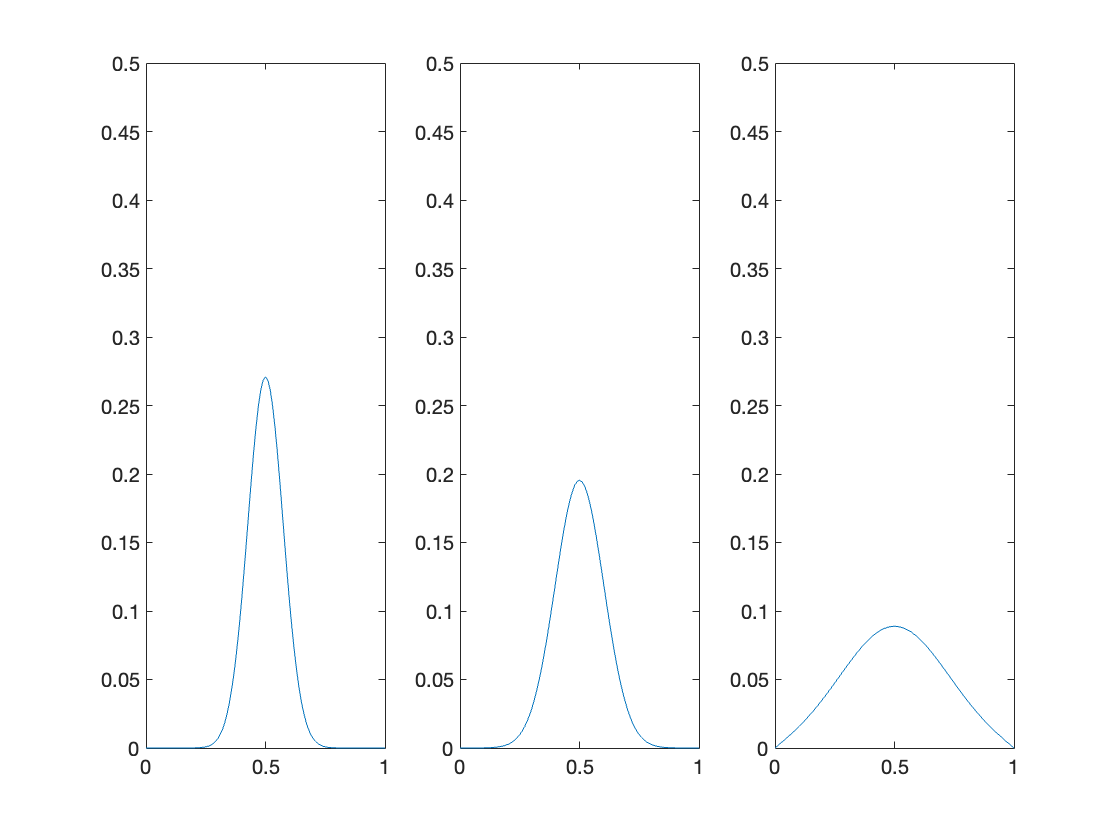
\includegraphics[scale = 0.25]{exact_solution.png}\\
CN with r=1\\
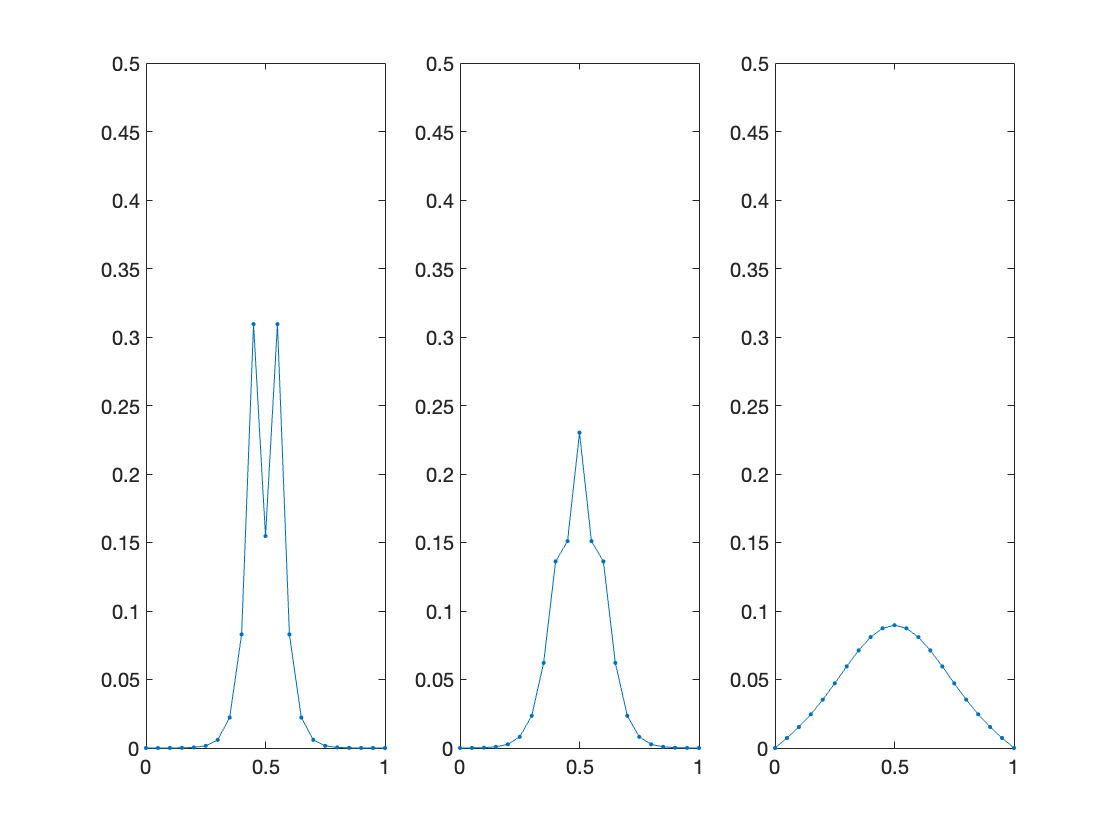
\includegraphics[scale = 0.25]{CN_1.png}\\
CN with r=2\\
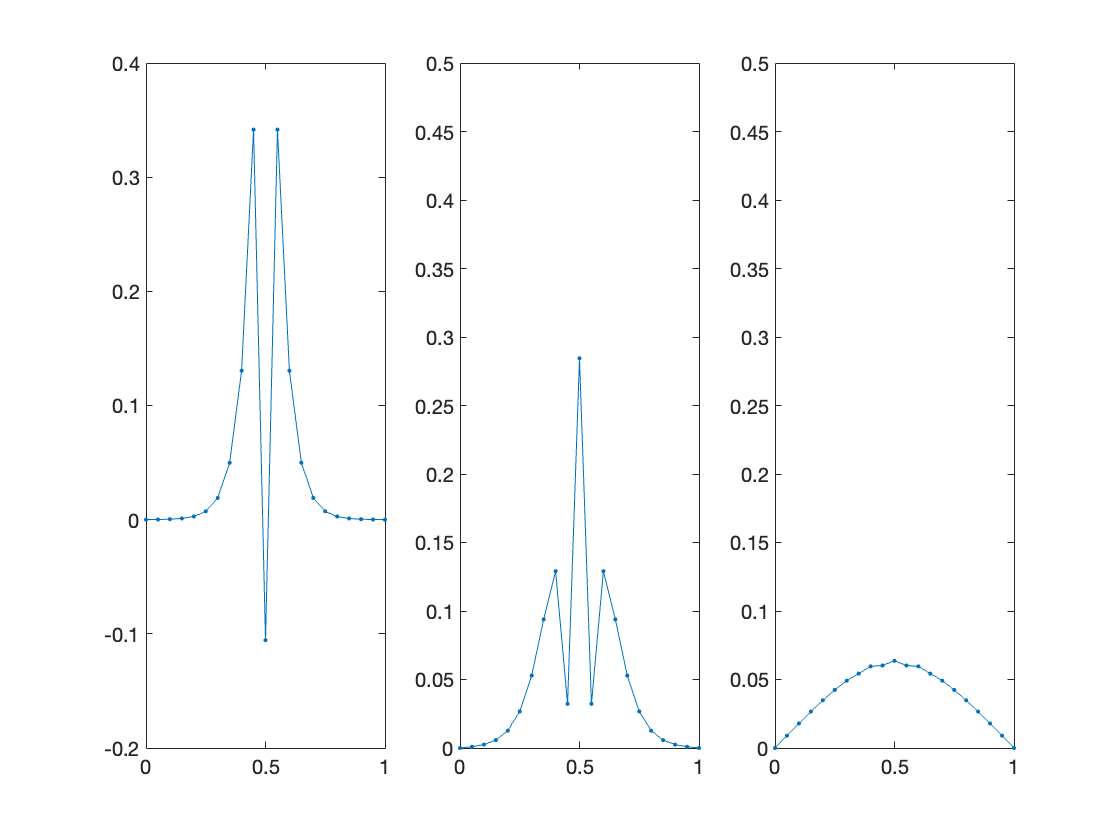
\includegraphics[scale = 0.25]{CN_2.png}\\
BTCS with r=1\\
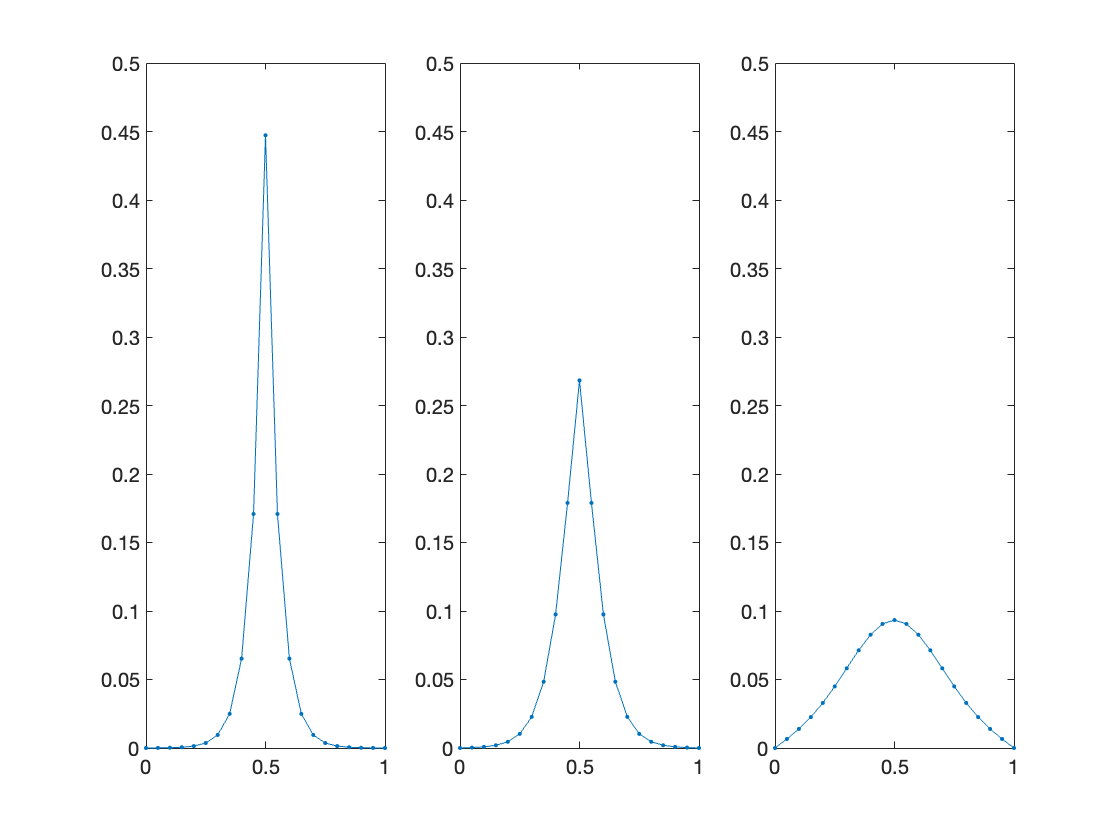
\includegraphics[scale = 0.25]{BTCS_1.png}\\
collocation with r=1\\
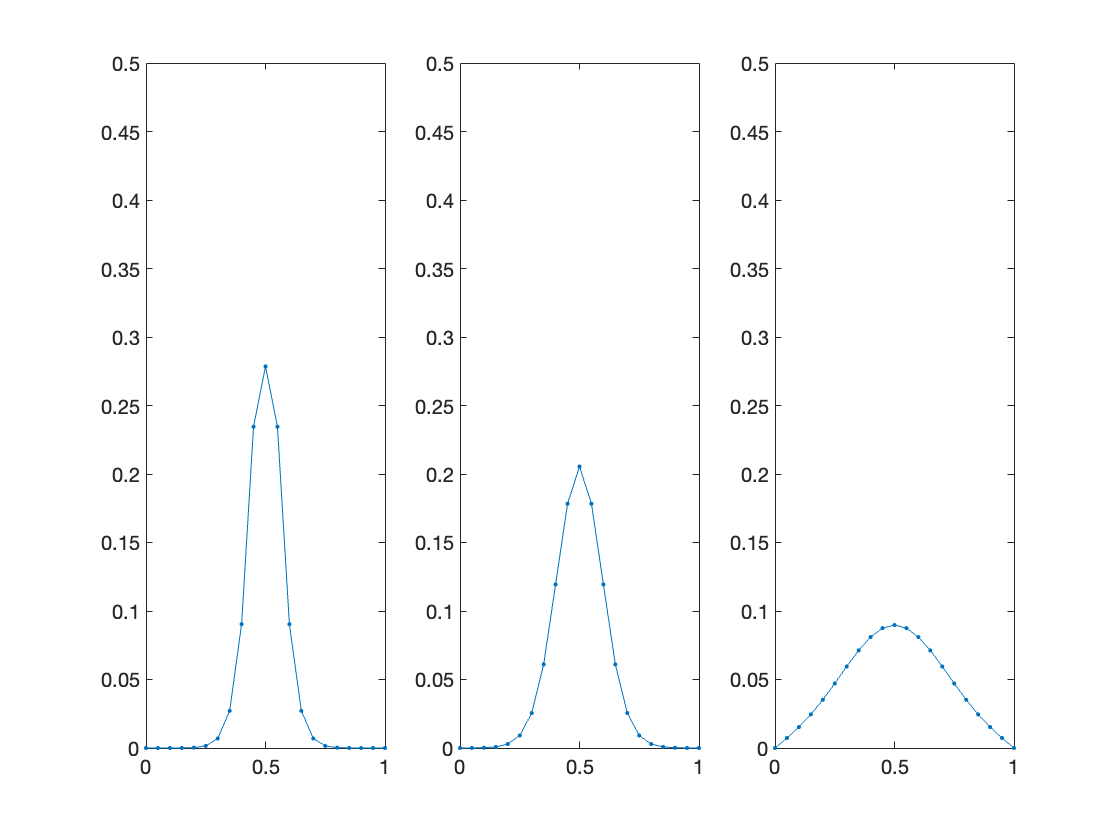
\includegraphics[scale = 0.25]{collocation_1.png}\\
BTCS with $r=\frac{1}{2h}$\\
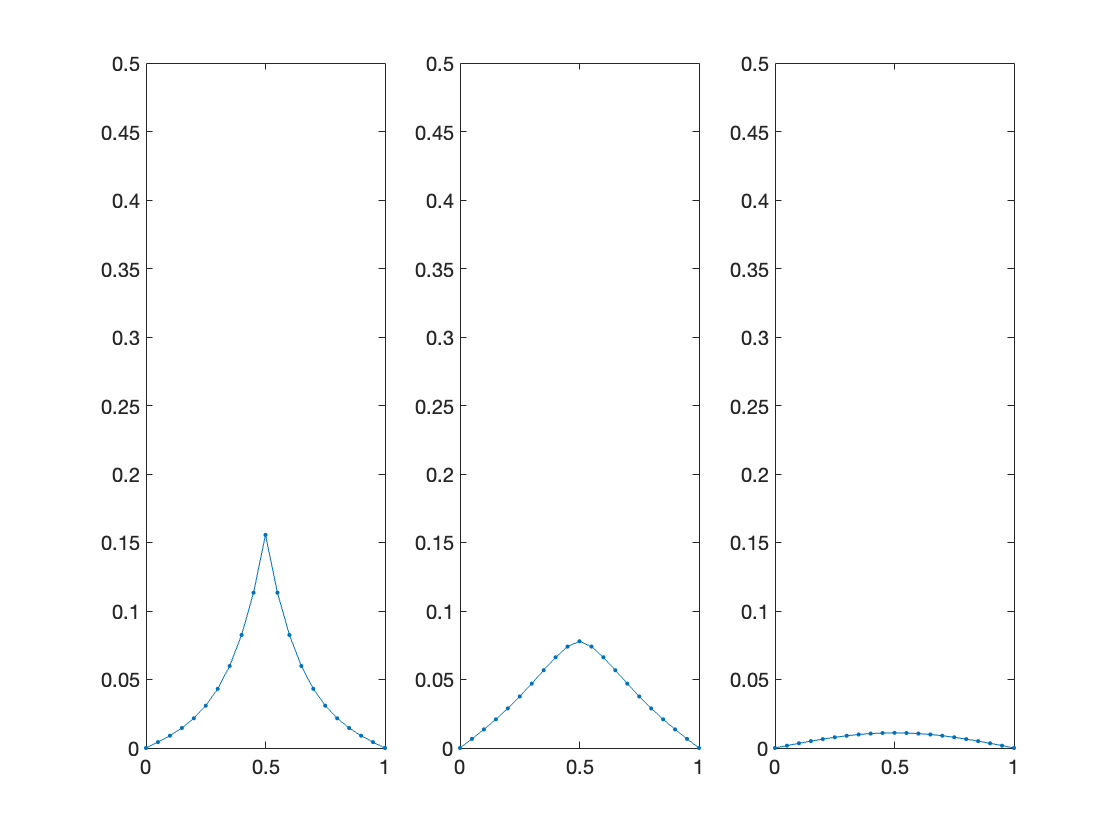
\includegraphics[scale = 0.25]{BTCS_2h.png}\\
collocation with $r=\frac{1}{2h}$\\
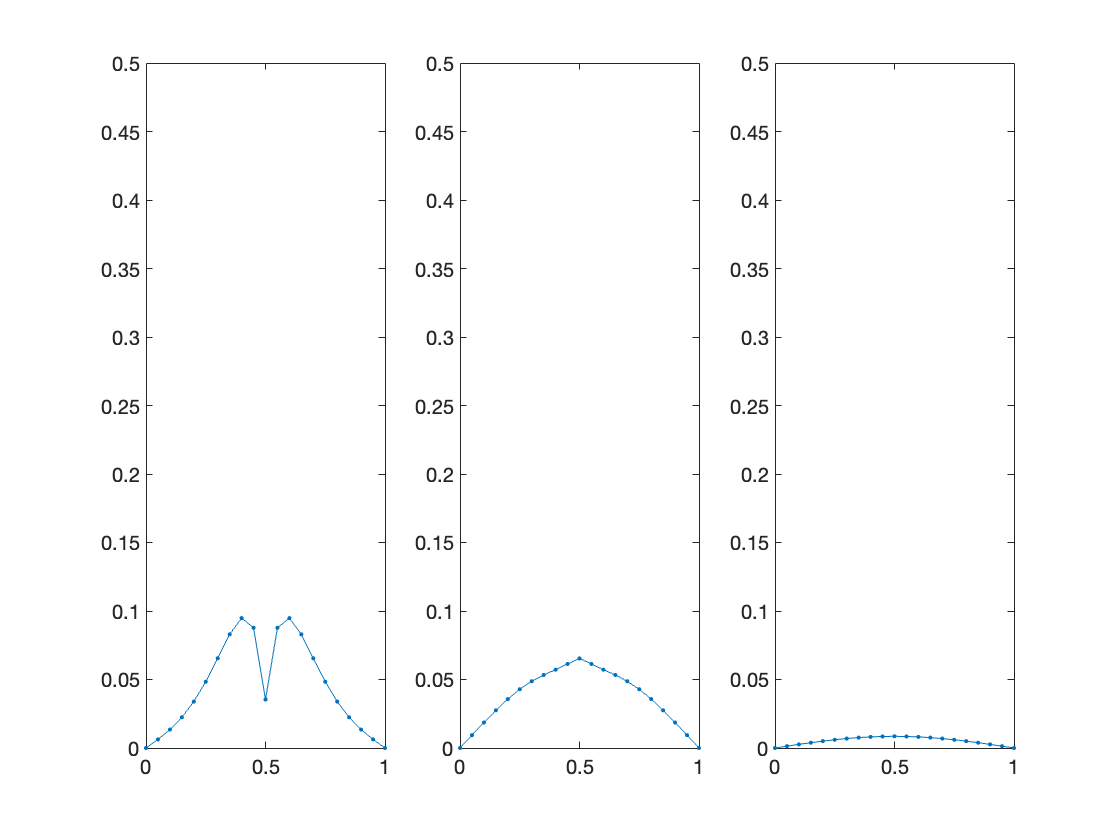
\includegraphics[scale = 0.25]{collocation_2h.png}\\
FTCS with r=1\\
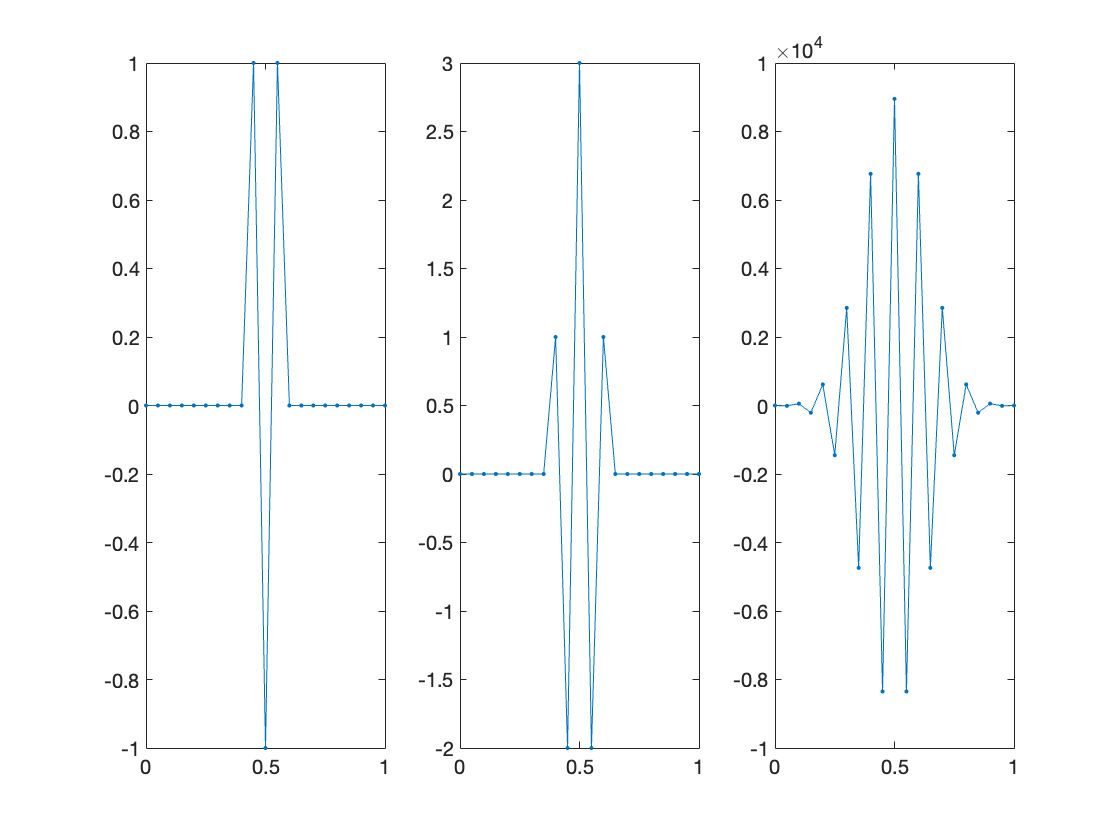
\includegraphics[scale = 0.25]{FTCS_1.png}\\
FTCS with $r=\frac{1}{2}$\\
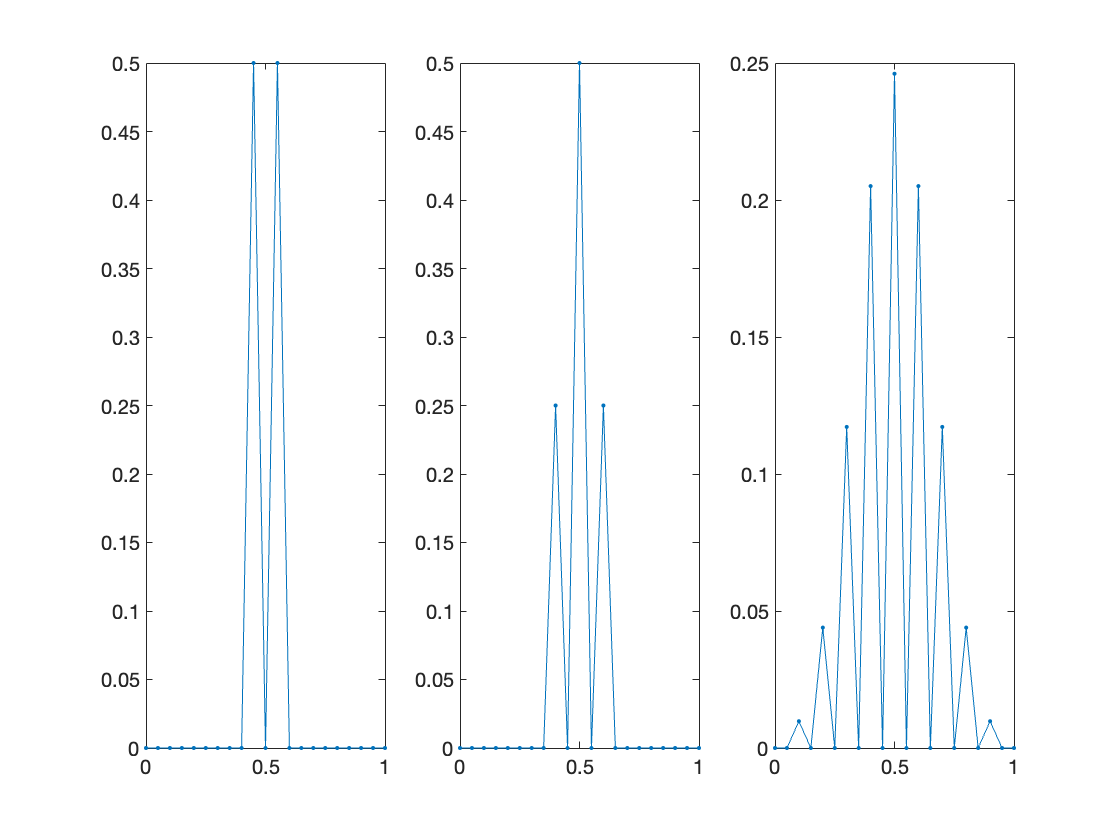
\includegraphics[scale = 0.25]{FTCS_2.png}\\
1-stage Gauss-Legendre RK method with r=1\\
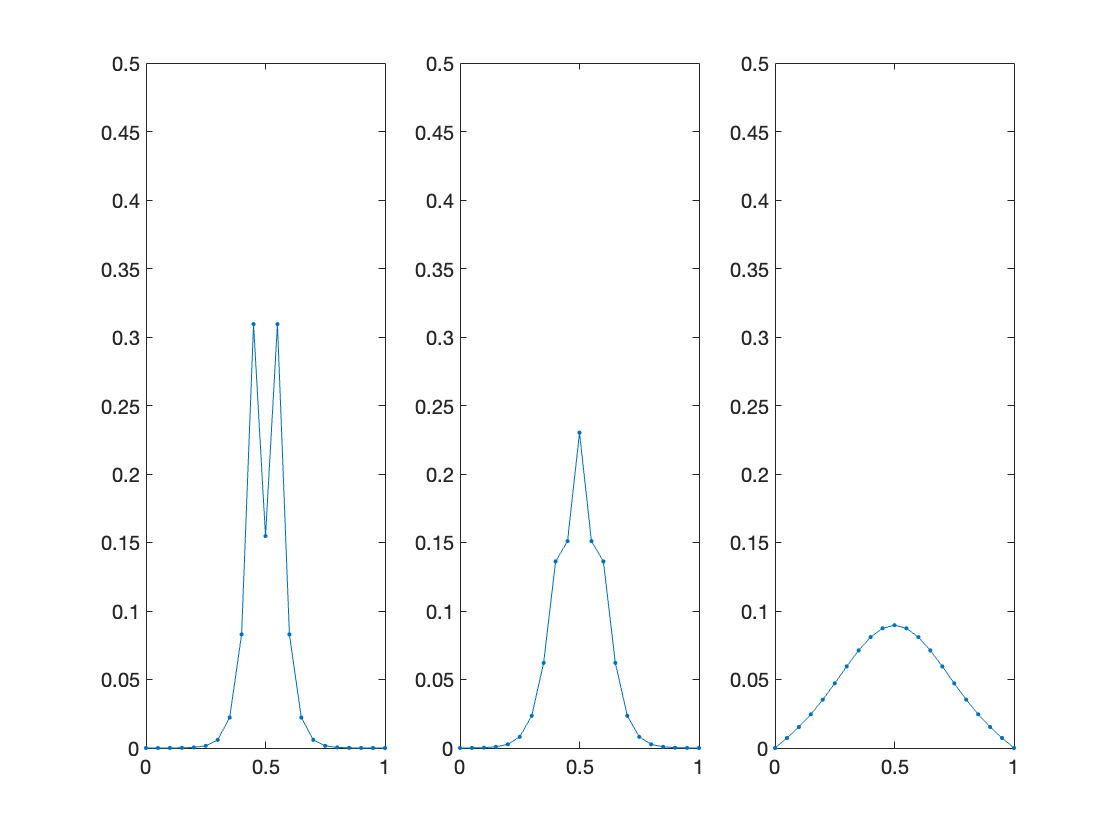
\includegraphics[scale = 0.25]{GS_1.png}\\
1-stage Gauss-Legendre RK method with $r=\frac{1}{2h}$\\
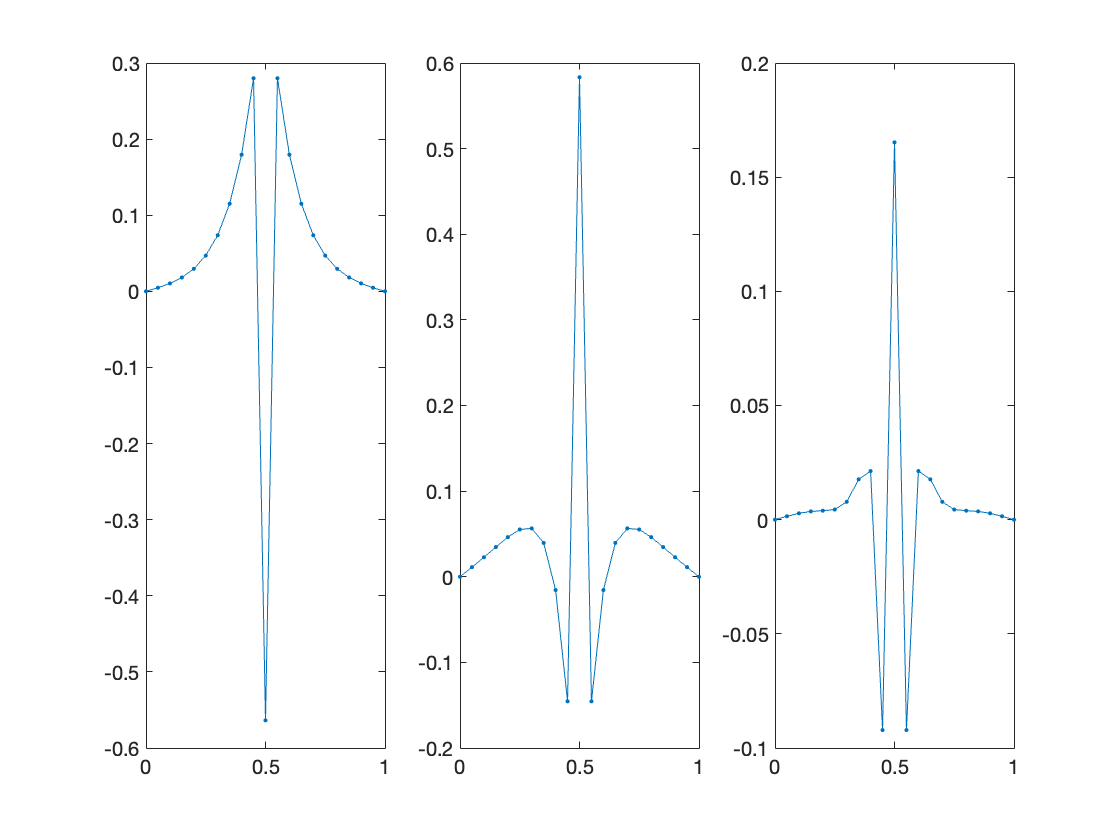
\includegraphics[scale = 0.25]{GS_2.png}\\
\indent 对于BTCS和collocation method方法在$r=\frac{1}{2h}$而言,能够明显的发现其图像变化的更快了,特别是可以发现它们在第二步的时候得到的结果与$r=1$时在第十步得到的结构一致,这是因为对于同一个方法的r的改变在h不变的情况下实际上是对k的改变,在$r=1$时,$k=h^2=\frac{1}{400}$,在$r=2$时,$k=\frac{h}{2}=\frac{1}{40}$,因此会导致前一种情况经过了10步之后在达到后一种情况2步的情况。\\
\indent 对于FTCS方法而言,将其视为一种$\theta-method$有$\theta=0$,因此在$r=1$时不满足11.36的条件,得到不11.36的结论,最终导致震荡,而在$r=\frac{1}{2}$时可以满足相应的条件从而得到相应的结论。\\
\indent 对于1-stage Guass-Legendre RK method,由于其本身不是L-stable的,因此会导致它的震荡。并且随着时间尺度的减小从某种意义上来说它的L-stable越弱,震荡在一定的步数内还存在




\end{document}